% E0240 Project 1, Phase-1 problem statement (due 22 September 2026).
% NOTE: the "Group members" line in the title block is a placeholder:
% fill in teammate names and SR numbers, or delete the line, before submission.
% Table 1 remains a planning/representative parameter table for Phase-1; measured
% real-system values are incorporated in later validation analysis.
\documentclass[conference]{IEEEtran}
\usepackage{amsmath,amssymb}
\usepackage{microtype}
\usepackage{booktabs}
\usepackage{tikz}
\usetikzlibrary{arrows.meta,positioning,calc}
\usepackage[hidelinks]{hyperref}
\usepackage[numbers,sort&compress]{natbib}

% Customise abstract delimiter to avoid em-dash
\makeatletter
\def\abstract{\normalfont
  \if@twocolumn
    \@IEEEabskeysecsize\bfseries\textit{\abstractname}:\space\relax
  \else
    \bgroup\par\addvspace{0.5\baselineskip}\centering\vspace{-1.78ex}\@IEEEabskeysecsize\textbf{\abstractname}\par\addvspace{0.5\baselineskip}\egroup\quotation\@IEEEabskeysecsize
  \fi\@IEEEgobbleleadPARNLSP}
\makeatother

\title{A Queueing-Network Simulator for an LLM Inference Serving Pipeline}
\author{\IEEEauthorblockN{Vaibhav Mahore (23631), [Name (SR No.)], [Name (SR No.)]}\IEEEauthorblockA{UG BTech (M\&C), Department of Computer Science and Automation\\
Indian Institute of Science, Bangalore}}

\begin{document}
\maketitle

\begin{abstract}
In this project, our team develops a cycle-driven discrete-time queueing-network simulator for an LLM inference serving pipeline. We model the serving stack as a three-station chain consisting of a deterministic tokenizer, a batching scheduler, and parallel GPU decode workers. We verify the implementation analytically against discrete-time closed forms and ground service parameters in empirical Tesla T4 GPU measurements. This report motivates our queueing abstraction, formalizes the network model, and presents our two-layer validation plan.
\end{abstract}

\section{Why an LLM Inference Serving Pipeline}
Large language model (LLM) inference serving operates under strict real-time constraints: users directly experience time-to-first-token and subsequent token delivery pace. Serving systems must satisfy tight latency targets while coping with unpredictable arrival bursts and variable prompt workloads.

Behind the API, modern serving stacks such as vLLM~\cite{kwon2023vllm} behave fundamentally as a sequence of queues. Incoming requests are tokenized, queued until an execution batch forms, and decoded on GPU workers whose runtime depends on generated token counts. User-visible latency is dominated by queueing delay (admission wait, batch accumulation, and worker contention). Our team therefore adopts time-average queue occupancy as the primary performance metric, directly connecting system state to user-perceived quality of service~\cite{zheng2023response}.

Batching creates an inherent throughput-versus-delay trade-off. Larger batches improve GPU utilization, but individual requests wait longer for batches to fill~\cite{yu2022orca}. Capturing this trade-off across batch caps, timeouts, and worker allocations is naturally suited to queueing models. Simulating these dynamics enables our team to study stability boundaries and queue buildup far more efficiently than benchmarking on expensive shared clusters.

\section{Related Work}
Recent LLM systems research focuses heavily on reducing latency and managing memory. Orca~\cite{yu2022orca} pioneered iteration-level scheduling to break requests out of static batches dynamically. vLLM~\cite{kwon2023vllm} developed PagedAttention to eliminate KV-cache fragmentation, supporting larger effective batches. FlexGen~\cite{sheng2023flexgen} analyzed high-throughput single-GPU serving via memory hierarchy offloading. At the simulation level, Vidur~\cite{agrawal2024vidur} replays profiled GPU execution traces to model cluster-level scheduling. Our team's approach is complementary: rather than profiling operator execution, we abstract the pipeline as a three-station queueing network. We validate our engine analytically against discrete-time closed forms~\cite{mor2006discrete} and calibrate service scaling using empirical GPU measurements, enabling fast, exhaustive sweeps across scheduler parameters.

\section{The Queueing Network Abstraction}
We model the LLM serving pipeline as an open, three-station feedforward queueing network with designated arrival and service parameters (Figure~1). Requests travel through each station sequentially. In steady state, each station sees the same average injection rate $\lambda$ (requests per cycle). External arrivals follow a Bernoulli process: in each discrete cycle, a new request arrives with probability $\lambda$.

\begin{figure}[!t]
\centering
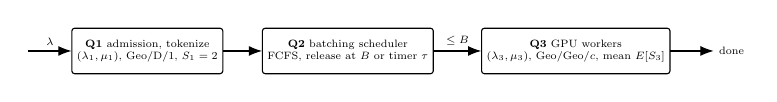
\begin{tikzpicture}[>=Latex, font=\scriptsize, scale=0.55, transform shape,
  stn/.style={draw, rounded corners=1pt, minimum width=3.1cm, minimum height=1.05cm, align=center}]
\node[stn] (q1) {\textbf{Q1} admission, tokenize\\ $(\lambda_1,\mu_1)$, Geo/D/1, $S_1=2$};
\node[stn,right=0.9cm of q1] (q2) {\textbf{Q2} batching scheduler\\ FCFS, release at $B$ or timer $\tau$};
\node[stn,right=1.1cm of q2] (q3) {\textbf{Q3} GPU workers\\ $(\lambda_3,\mu_3)$, Geo/Geo/$c$, mean $E[S_3]$};
\draw[->] ($(q1.west)+(-1.0,0)$) -- node[above]{$\lambda$} (q1.west);
\draw[->] (q1) -- (q2);
\draw[->] (q2) -- node[above]{$\le B$} (q3);
\draw[->] (q3.east) -- ++(1.0,0) node[right]{done};
\end{tikzpicture}
\caption{The LLM serving pipeline as a three-station queueing network.}
\end{figure}

\textbf{Q1: Admission and tokenization.} A single server with deterministic service time $S_1 = 2$ cycles per request (request validation, formatting, and tokenization), following Geo/D/1 with $\mu_1 = 1/S_1$. Setting $S_1 = 2$ enables direct verification against discrete-time closed forms.

\textbf{Q2: Batching scheduler.} A FCFS buffer releasing requests as a batch when $B$ requests accumulate or the oldest request has waited $\tau$ cycles. With $B = 1$, Q2 becomes a zero-delay pass-through buffer used for baseline validation. Our model captures static batching; continuous batching is an extension.

\textbf{Q3: GPU workers.} A pool of $c$ identical parallel workers serving one batch at a time, where all batch requests share the service duration. The baseline abstraction uses geometric batch service with mean $E[S_3]$ cycles (Geo/Geo/$c$), representing variable decode length under memoryless completion probability $p_s = 1/E[S_3]$.

\textbf{Simplifying assumptions.} Requests traverse the pipeline once without feedback; batching modifies waiting times rather than total compute; workers are homogeneous and non-preemptive; external arrivals are memoryless Bernoulli trials.

Station $i$ is stable when $\rho_i = \lambda E[S_i] < 1$. Because requests are conserved along the path, $\lambda_i = \lambda$ throughout. The binding conditions are $2\lambda < 1$ at Q1 and $\lambda E[S_3]/c < 1$ at Q3; Q2 is stable whenever Q3 is. Table~1 summarizes representative parameters mapped to model cycles.

\begin{table}[!t]
\centering\scriptsize
\caption{Representative parameters mapped to model cycles.}
\setlength{\tabcolsep}{2.5pt}
\begin{tabular}{@{}p{1.25cm}p{1.85cm}p{2.65cm}p{1.45cm}@{}}
\toprule
Quantity & Real system & Model value & Provenance \\
\midrule
Sched.\ tick & 10--50\,ms per pass & one cycle & representative \\
Arrivals & request stream & Bernoulli($\lambda$), sweep $\lambda \in [0.05, 0.45], 0.49$ & validation \\
Batch cap $B$ & 8--32 req/batch & $B \in \{1,4,8,16,32\}$ ($B=1$ valid.) & representative \\
Wait timer $\tau$ & a few ticks & $\tau \in \{1,2,5,10\}$ cycles & representative \\
Decode len.\ & variable, tens of tokens & geometric, mean $E[S_3]=20$ (swept) & geometric law \\
Tokenizer & small fixed overhead & $S_1 = 2$ cycles, deterministic & std.\ validation \\
GPU slots $c$ & 8--32 seqs/GPU & $c=1$ validation; 2--32 expt.\ & representative \\
\bottomrule
\end{tabular}
\end{table}

\section{Key Performance Metric and Method}
Across stations, we track time-average queue occupancy $L_{q,i} = (1/T)\sum_t Q_i(t)$, average waiting delay $(\sum D_i)/n$, and server utilization (fraction of busy cycles). We verify accounting consistency by checking that measured utilization matches theoretical intensity $\rho_i = \lambda E[S_i]$ (or $\lambda E[S_3]/c$ at Q3) and that per-station delay satisfies $W = L_q/\lambda$. Total end-to-end delay is the sum of delays across all three stations.

Our team implements the simulator using a cycle-driven discrete-event loop: time advances in uniform increments of one cycle. Each cycle, the engine (i)~admits an arrival with probability $\lambda$ using uniform draw $U \in [0,1)$, (ii)~decrements countdowns for busy servers, (iii)~dispatches released batches or head-of-line requests to idle workers, and (iv)~increments occupancy and utilization counters. Random variates are generated via inverse transform: Bernoulli arrivals via $U \le \lambda$ and geometric service via $U < p_s$. We implemented the simulator in Python, generate plots with matplotlib, and fix the random seed (20260922) to guarantee reproducibility.

\section{Validation and Plan of Action}
\textbf{Quantitative goal.} Our team targets agreement between simulated metrics and analytical closed forms within 1\% for $\lambda \le 0.45$ over $10^7$ cycles. For empirical calibration, we target held-out GPU batch time prediction within 15\% MAPE.

\textbf{Layer 1: Analytical verification.} With Q2 in pass-through mode ($B=1, c=1$), we verify single-station behavior against discrete-time closed forms. For deterministic service, $W_q = \rho(S-1)/(2(1-\rho))$ and $L_q = \lambda W_q = \lambda^2 S(S-1)/(2(1-\lambda S))$, which simplifies to $L_q = \lambda^2/(1-2\lambda)$ when $S=2$. For geometric service with $E[S_3]=2$, we verify $L_q = 2\lambda^2/(1-2\lambda)$, confirming the exact factor-2 variance penalty. We also confirm $\rho_i = \lambda E[S_i]$, $W = L_q/\lambda$, flow conservation, and convergence across run lengths from $10^3$ to $10^7$ cycles.

\textbf{Layer 2: Empirical GPU calibration.} To ground model parameters in hardware, our team collected batched inference measurements on a Tesla T4 GPU running Qwen 2.5-1.5B across $B \in \{1,\dots,32\}$. We calibrate service scaling on split $\{1,4,16\}$ and evaluate predictive accuracy on held-out batch sizes $\{2,8,32\}$. Formalizing the physical millisecond-to-cycle mapping and Q3 parameter calibration is ongoing Phase-2 work.

\textbf{Planned experiments.} We conduct two experimental campaigns: first, evaluating geometric versus deterministic service across worker counts $c \in \{1,2\}$ to quantify variability penalties and parallelism benefits; second, sweeping batch capacity $B$ and timeout $\tau$ at fixed loads to map the batching scheduler trade-off.

\bibliographystyle{IEEEtranN}
\bibliography{phase1_refs}

\end{document}
